\documentclass[hyperref={colorlinks=false},compress,handout,10pt]{beamer}

\usepackage{tikz}
%\usepackage[active,tightpage,psfixbb]{preview}

%\PreviewEnvironment{pgfpicture}

%\setlength\PreviewBorder{0pt}

\newlength{\wideitemsep}
\setlength{\wideitemsep}{\itemsep}
\addtolength{\wideitemsep}{100pt}
\let\olditem\item
\renewcommand{\item}{\setlength{\itemsep}{0.5\baselineskip}\olditem}


\def\LaTeXs{\LaTeX\ }

%\usepackage{tikz}
%\usepackage{pgfplots}

%\usetikzlibrary{arrows,calc}
%%%<
%\usepackage{verbatim}

%\usetikzlibrary{calc,fadings,decorations.pathreplacing,backgrounds}
%% helper macros

%\tikzset{variable/.default=}  

%\tikzset{%
%    add/.style args={#1 and #2}{ to path={%
%    ($(\tikztostart)!-#1!(\tikztotarget)$)--($(\tikztotarget)!-#2!(\tikztostart)$)%
%\tikztonodes},add/.default={.2 and .2}}
%}  


%\tikzset{%
%    >=latex,
%    inner sep=0pt,
%    outer sep=2pt,
%    mark coordinate/.style={inner sep=0pt,outer sep=0pt,minimum size=2pt,
%    fill=black,circle}%
%}





\usetheme{Singapore}
\usecolortheme{lily}
%\usecolortheme[rgb={0,0.17,0.45}]{structure} 
%\usecolortheme[rgb={.855,.647,.125}]{structure} 
\usefonttheme[onlymath]{serif}

%\usepackage{beamerarticle}
\usepackage{listings}
\lstset{
basicstyle=\footnotesize\ttfamily,
%numbers=left,
frame=bottomline,
framextopmargin=50pt,
}


\usepackage{amsmath,amsthm,amssymb}



\usepackage{float}
\floatstyle{boxed}
\usepackage{colortbl}
\usepackage{mathpazo}
%\usepackage[small]{eulervm}
%\usepackage[tiling]{pst-fill}
\usepackage{graphicx}
\usepackage{movie15}
\usepackage{bm}
\usepackage{verbatim}
\usepackage{comment}
\usepackage{caption}
\usepackage{subcaption}
\captionsetup[subfigure]{labelformat=empty}
\captionsetup[figure]{labelformat=empty}
%\usepackage[hang,nooneline]{subfigure}
%\usepackage[nooneline]{subfigure}
%\usepackage[OT2,T1]{fontenc}
%\usepackage{pgf,pgfarrows,pgfautomata,pgfheaps,pgfnodes,pgfshade}
%\usepackage{animate}
%\DeclareGraphicsRule{.tif}{png}{.png}{`convert #1 `dirname #1`/`basename #1 .tif`.png}
\graphicspath{{./images/}}
%\renewcommand{\thesubfigure}{}

\newcommand{\mygreen}{\color{green!50!black}}
\newcommand{\myblue}{\color{blue}}
\newcommand{\myred}{\color{red}}
\newcommand{\mycolor}{\color{red}{c}\color{blue}{o}\color{green}{l}\color{orange}{o}\color{cyan}{r}}
\newcommand{\mysize}{\scriptsize{s}\small{i}\normalsize{z}\Large{e}}
\newcommand{\myshape}{\textcircled{s}\textit{h}\texttt{a}\textsf{p}\textsc{e}}

\newcommand{\E}{\mathcal{E}}
\newcommand{\A}{\mathcal{A}}
\newcommand{\mb}{\mathbf}

\newcounter{cnt}
\setcounter{cnt}{0}


%\setbeamercolor*{titlelike}{parent=palette tertiary} 
\xdefinecolor{titlecolor}{rgb}{.855,.647,.125}
%\setbeamercolor{titlelike}{parent=titlecolor}
\setbeamercolor{frametitle}{fg=titlecolor}
\setbeamerfont{frametitle}{series=\bfseries}
%\setbeamercolor{frame title alerted}{use=alerted text,fg=titlecolor,bg=alerted text.fg!75!bg}
%\setbeamercolor{frame title example}{use=example text,fg=titlecolor,bg=example text.fg!75!bg}
%\setbeamercolor{math text}{fg=green!50!black}
\setbeamercolor{normal text in math text}{parent=math text}

\setbeamertemplate{navigation symbols}{} %gets rid of navigation symbols
\setbeamertemplate{mini frames}{}
\setbeamertemplate{footline}[frame number]
\beamertemplateshadingbackground{blue!5}{yellow!10}

\title{{\color{blue} \LARGE 550.400: Mathematical Modeling and Consulting\newline} }

\subtitle{{\color{red} \large Lecture Notes} }

\author{ 
    {\bf{Instructor:}} \\ 
Dr.~N.~H.~Lee \\ 
    \vspace{5pt}
} 
\institute{JHU AMS 2012 FALL}


%\date{\mygreen \today} % \\ Sparks, Nevada}

\date{\mygreen Last Compiled on \today} 

\begin{document}

\begin{frame}[plain]
  \titlepage
\end{frame}



\begin{frame}
  \frametitle{Outline}
  \tableofcontents
\end{frame}


\section{Class Info.}

\begin{frame}
    \frametitle{Syllabus}
    \begin{itemize}
        \item Grade Policy
        \item Attendance
        \item \emph{Tentative} Schedule
        \item Blackboard
        \item Misc.
    \end{itemize}
\end{frame}

\begin{frame}
    \frametitle{OH Location}
    \begin{figure}
        \caption{Clark Hall 320B}
        \begin{center}
            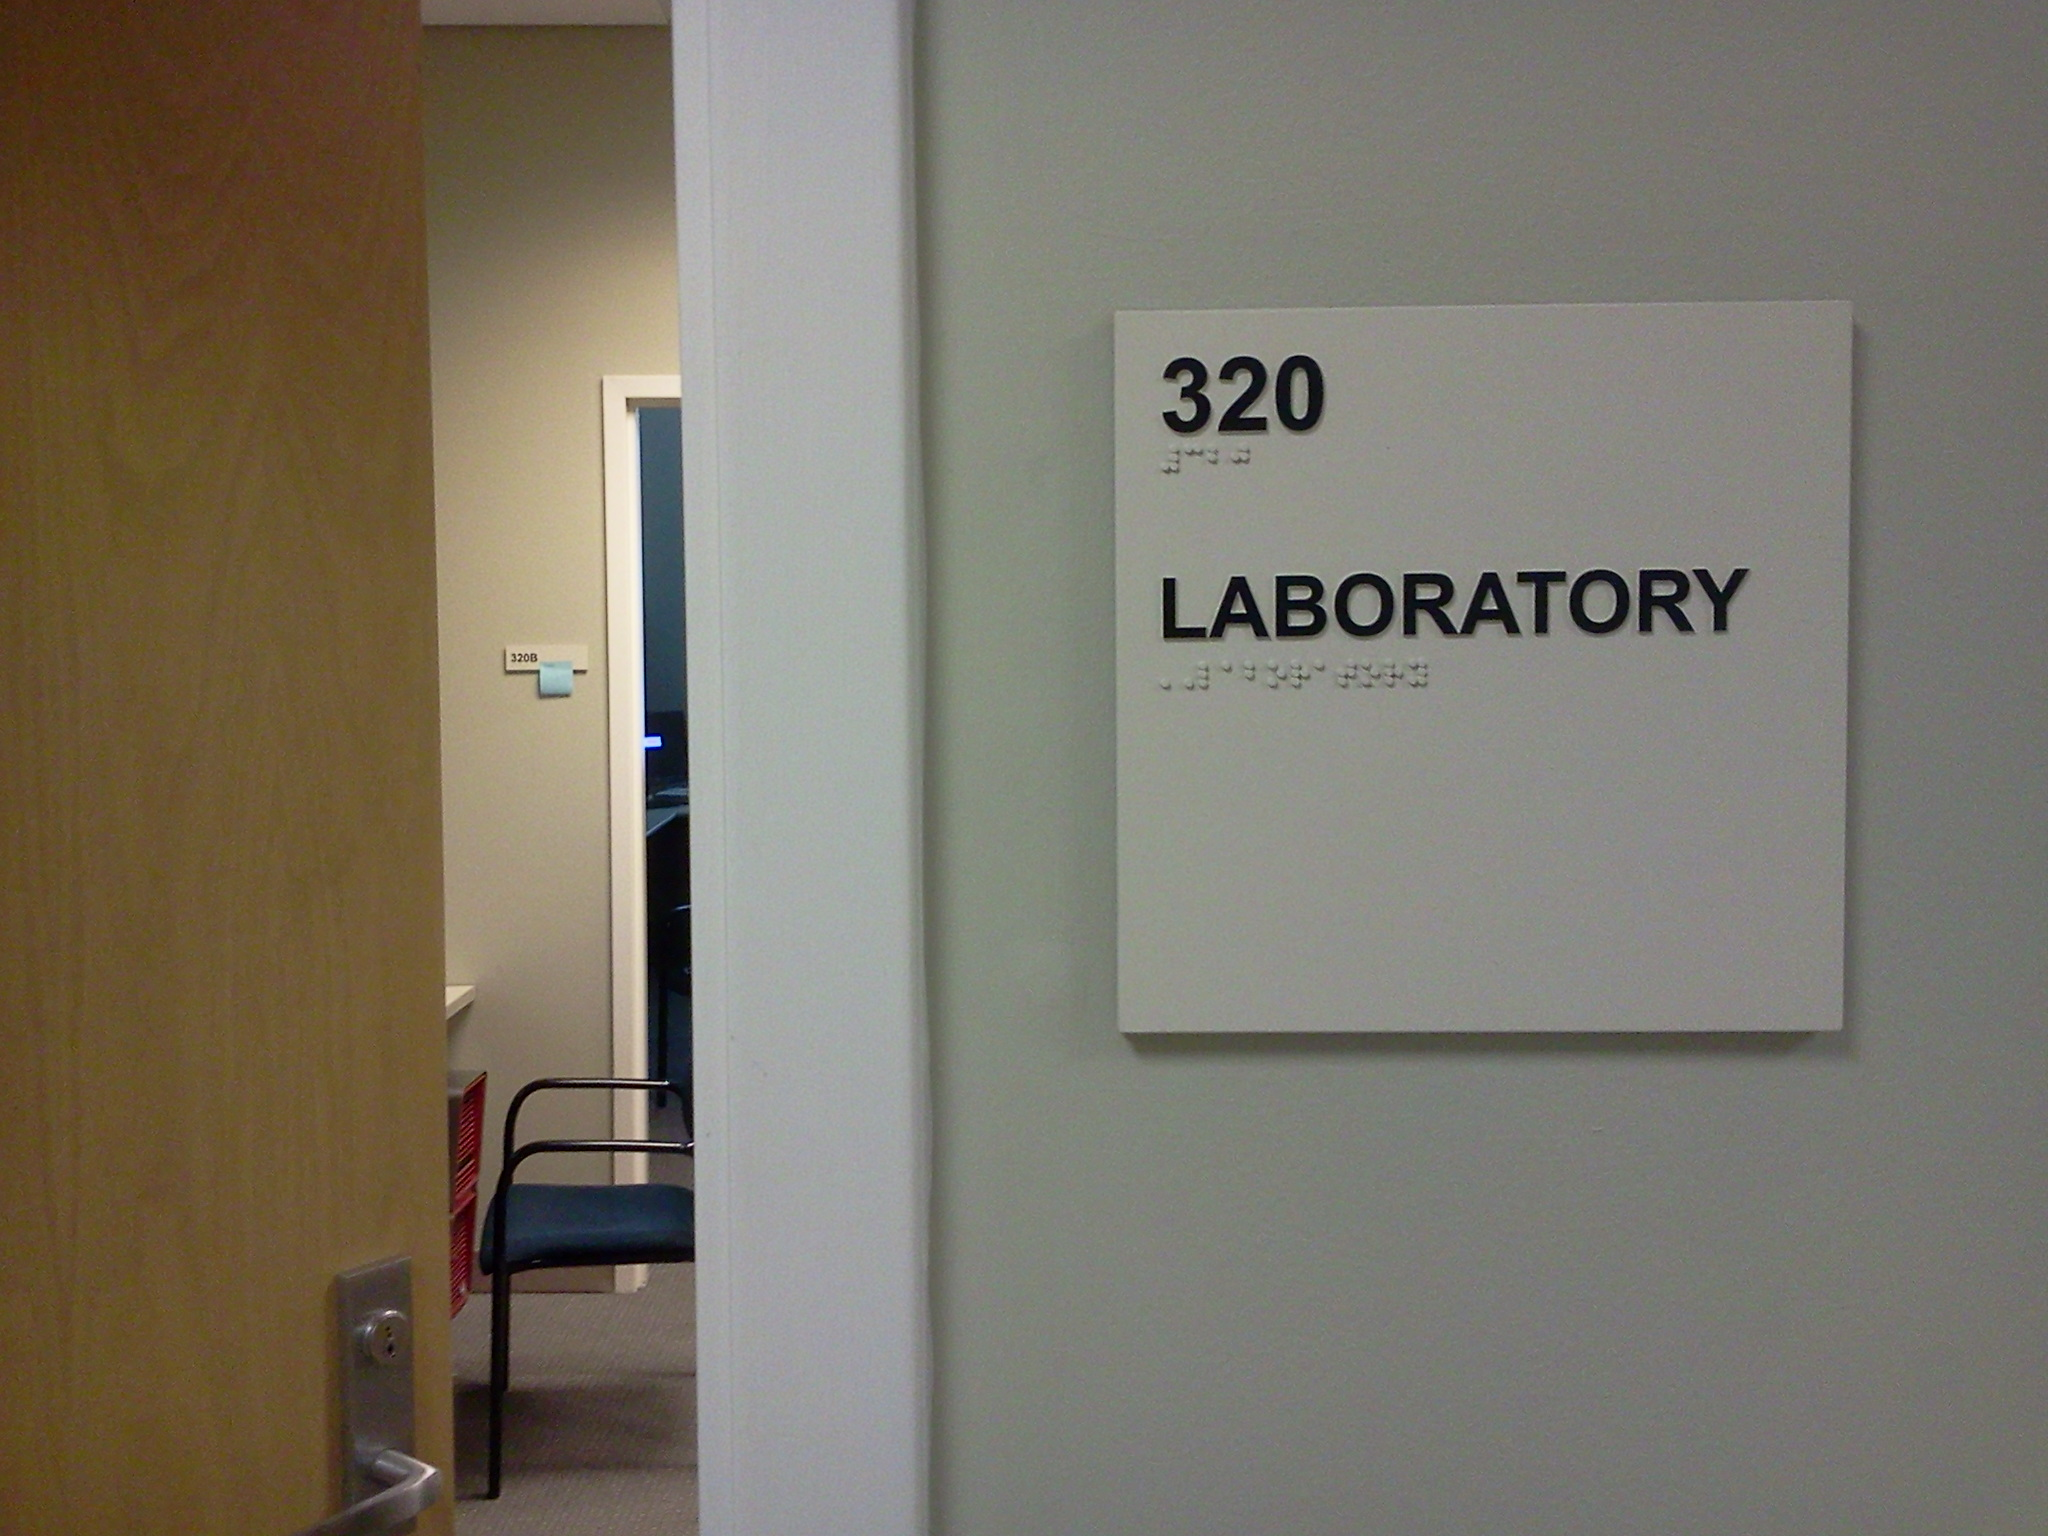
\includegraphics[width=0.75\textwidth]{images/Clark320B.jpg}
        \end{center}
        \label{fig:ClarkHall320B}
    \end{figure}
\end{frame}

\begin{frame}[fragile]
    \frametitle{Course Book Reserve}
    \vskip0.5in
    \begin{center}
        \href{https://catalyst.library.jhu.edu/reserves/13812}{JHU Library Reserve Service}
    \end{center}
\end{frame}

\begin{frame}
    \frametitle{Presentations in this class}
    \begin{figure}
        \caption{For your presentation recording needs}
        \href{https://know.it.jhu.edu/display/TECHCLASS/Homewood+Campus}{
        
\includegraphics[width=0.7\textwidth]{images/BLC2006.jpg}}
    \end{figure}
\end{frame}

\begin{frame}[fragile]
    \frametitle{Unofficial Way to Access the Course Folder}
    \vskip0.5in
    \begin{center}
        \href{http://cis.jhu.edu/~nhlee/550400.html/}{
            \url{http://cis.jhu.edu/~nhlee/550400.html/}
        }
    \end{center}
\end{frame}


\section{Theory}

\subsection{Writing about numbers}
\begin{frame}
    \frametitle{Seven Basic Principles}
     \begin{enumerate}
         \item Set the context 
         \item Choose effective examples and analogies
         \item Choose vocabulary to suit your readers
         \item Decide whether to present \#s in text, tables, or figures
         \item Report and interpret \#s in the text
         \item Specify the direction \emph{and} size of an association between variables
         \item For many \#s, summarize overall pattern 
     \end{enumerate}
\end{frame}


\subsection{Math. Modeling}


\begin{frame}
    \frametitle{Models and Reality}
    \begin{verse}
        The ultimate test of a model is how well it performs when 
        it is applied to the problem it was designed to handle.
    \end{verse}
    \vskip0.5in
    \begin{verse}
       A model is used, it may lead to incorrect predictions. The model is
       often modified, frequently discarded, and sometimes used anyway because
       it is better than nothing. This is the way science develops.  
    \end{verse}
\end{frame}

\begin{frame}
    \frametitle{Models and Reality}
    What makes Mathematical models useful? We must/have/have/have:
    \vskip0.1in
    \begin{itemize}
        \item formulate our ideas precisely and so are less likely to let implicit assumptions slip by,
        \item concise ``language'' which encourages manipulation,
        \item a large number of potential theorems available,
        \item high speed computers available for carrying out calculations.
    \end{itemize}
\end{frame}

\begin{frame}
    \frametitle{Properties of Models}
    As far as a model is concerned, the world can be divided into three parts:
    \vskip0.1in
    \begin{itemize}
        \item Things whose effects are neglected,
        \item Things that affect the model but whose behavior the model is not
            designed to study,
        \item Things the model is designed to study the behavior of. 
    \end{itemize}
\end{frame}
   
\subsection{Work Statement}
\begin{frame}
    \frametitle{A recurring theme}
    Frequently Recurring Elements of doing a Project in Industry:
    \vspace{7pt}
             \begin{enumerate}
                 \item Work Statement,
                 \item Midterm Presentation,
                 \item Progress Report,
                 \item Final Presentation,
                 \item Final Report.
             \end{enumerate}
    \begin{center}
        \href{http://www.ipam.ucla.edu/programs/rips2011/}{
        
\includegraphics[width=0.8\textwidth]{images/ipam}}        
    \end{center}
\end{frame}

\begin{frame}
    \frametitle{What is Work Statement?}
    \begin{itemize}
        \item The written proposal and definition of the project
            \vspace{1cm}
        \item Your consulting team's ``contract'' with the sponsor
            \vspace{1cm}
        \item It is ultimately given to the sponsor for review and signature
    \end{itemize}
\end{frame}



\begin{frame}
    \frametitle{What is Work Statement?}
It sets forth: 
    \begin{itemize}
        \item the nature of the project,
        \item the specific objectives of the project, 
        \item the result expected, 
        \item the ``deliverable'' for the project.
    \end{itemize}
\end{frame}

\begin{frame}
    \frametitle{What is Work Statement?}
    \begin{itemize}
        \item The scope of the project must be within the time table for the
            course
            \vspace{1cm}
        \item The deliverables are reasonable and appropriate
    \end{itemize}
\end{frame}

\begin{frame}
    \frametitle{What is Work Statement?}
    \begin{itemize}
        \item Given the nature of research, it should not include promises
            that your consulting team cannot be certain to achieve
            \vspace{1cm}
        \item It may be necessary after discussion and agreements among
            various parties to modify and renegotiate the work statement as 
            the project progresses
    \end{itemize}
\end{frame}

\begin{frame}
    \frametitle{Work Statement: Introduction}
    Describe:
    \begin{itemize}
        \item the purpose of the project,
        \item a brief introduction of the sponsoring organization,
        \item a suitably condensed statement of the problem,
        \item some discussion of the relevance of the project to the sponsor.
    \end{itemize}
\end{frame}

\begin{frame}[fragile]
    \frametitle{Work Statement: Introduction}
    The work statement should contain a short description 
    of your sponsor.  
    \vskip0.2in
    For the insurance redlining example, 
    \emph{U.S.~Commision on Civil Rights} would be the sponsor.
    \vskip0.2in
    \href{http://en.wikipedia.org/wiki/Boilerplate_%28text%29}{\emph{Boilerplating}} from the sponsor's webpage is often acceptable. 
    \vskip0.5in
    \begin{center}
        \href{http://www.usccr.gov/about/}{http://www.usccr.gov}
    \end{center}
\end{frame}

\begin{frame}   
    \frametitle{Work Statement: Problem Statement}
    \begin{verse}
        Can the insurance companies claim that the discrepancy is due to 
        greater risks in some zip codes?
    \end{verse}
    \vskip0.5in
    \begin{verse}
        The insurance companies could claim that they were denying insurance 
        in neighborhoods where they had sustained large fire-related losses
        and any discriminatory effect was a by-product of legitimate business
        practice.  
    \end{verse}
\end{frame}

\begin{frame}[fragile]
    \frametitle{Work Statement: Timeline \& Deliverable}
    \begin{verse}
        ``When I decide the time needed for the project,
        I first approximate the time that I might actually need, 
        and then, request the sponsor the double of the approximated time.''
    \end{verse}
    \vskip0.3in
    \begin{description}
        \item[From Team to Sponsor] Presentations, Reports, Special Softwares.
            \vskip0.5in
        \item[From Sponsor to Team] Regular meetings, Data \& Contingences,
            Code \& Code Documentation.
    \end{description}
\end{frame}



\section{Example}

\subsection{Random Bits}
\begin{frame}
    \frametitle{What is Mathematical Modeling?}
    \begin{figure}
            \centering
            \caption{
            \href{http://www.youtube.com/watch?feature=endscreen&v=UuXwYZ3AQU0&NR=1}
            {Money Ball}}
            \href{http://www.youtube.com/watch?v=WNlCBy07z08}{
            
\includegraphics[width=0.4\textwidth]{Moneyballs.jpg}
            }
            \label{fig:MondayBall} 
    \end{figure}
\end{frame}

\begin{frame}
    \frametitle{What is Mathematical Modeling?}
    \begin{figure}
        \centering
        \caption{
        \href{http://www.youtube.com/watch?v=Jzl39jqZjsw&feature=share&list=UUEWRMyobsgQG-PaC9ldME4A}{
        Trillion Dollar} 
        \href{http://www.youtube.com/watch?v=G17rx7H3DtI&feature=BFa&list=UUEWRMyobsgQG-PaC9ldME4A}{Bet}
        }
        \href{http://www.youtube.com/watch?v=dsrOXJwGwtk}{
        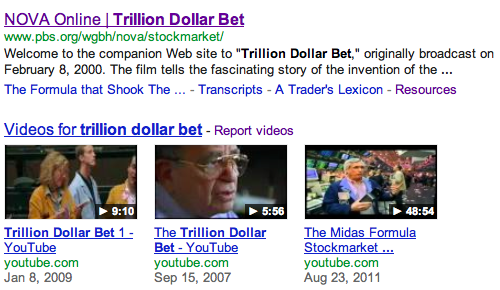
\includegraphics[width=\textwidth]{TrillionDollarBet.png}
        }
        \label{fig:LTCM}
    \end{figure}
\end{frame}

\begin{frame}
    \frametitle{What is Mathematical Modeling?}
    \begin{figure}
        \centering
        \caption{{LAPD Fighting Crime with Math}}
        \href{http://www.youtube.com/watch?v=HZ7fLuO7zb4}{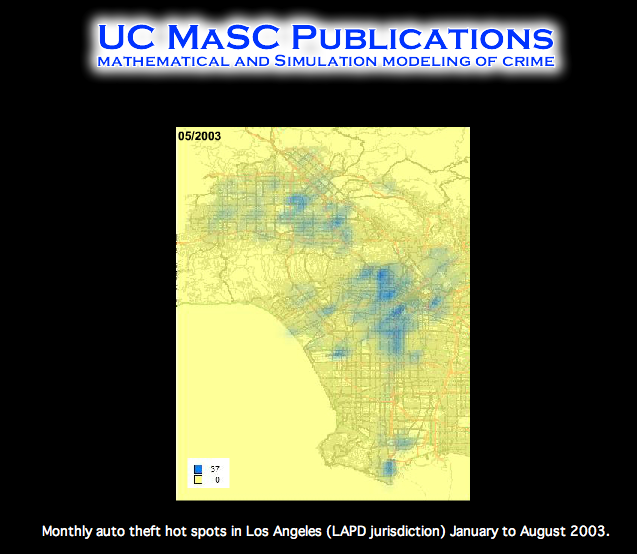
\includegraphics[width=0.6\textwidth]{LAPDUCLA.png}}
        \label{fig:LAPDUCLA}
    \end{figure}
\end{frame}

\begin{frame}[fragile]
    \frametitle{What is Mathematical Modeling?}
        \begin{figure}
            \centering
            \caption{Crime rates and religious beliefs}
            \href{http://www.economist.com/blogs/graphicdetail/2012/09/daily-chart/print}{
            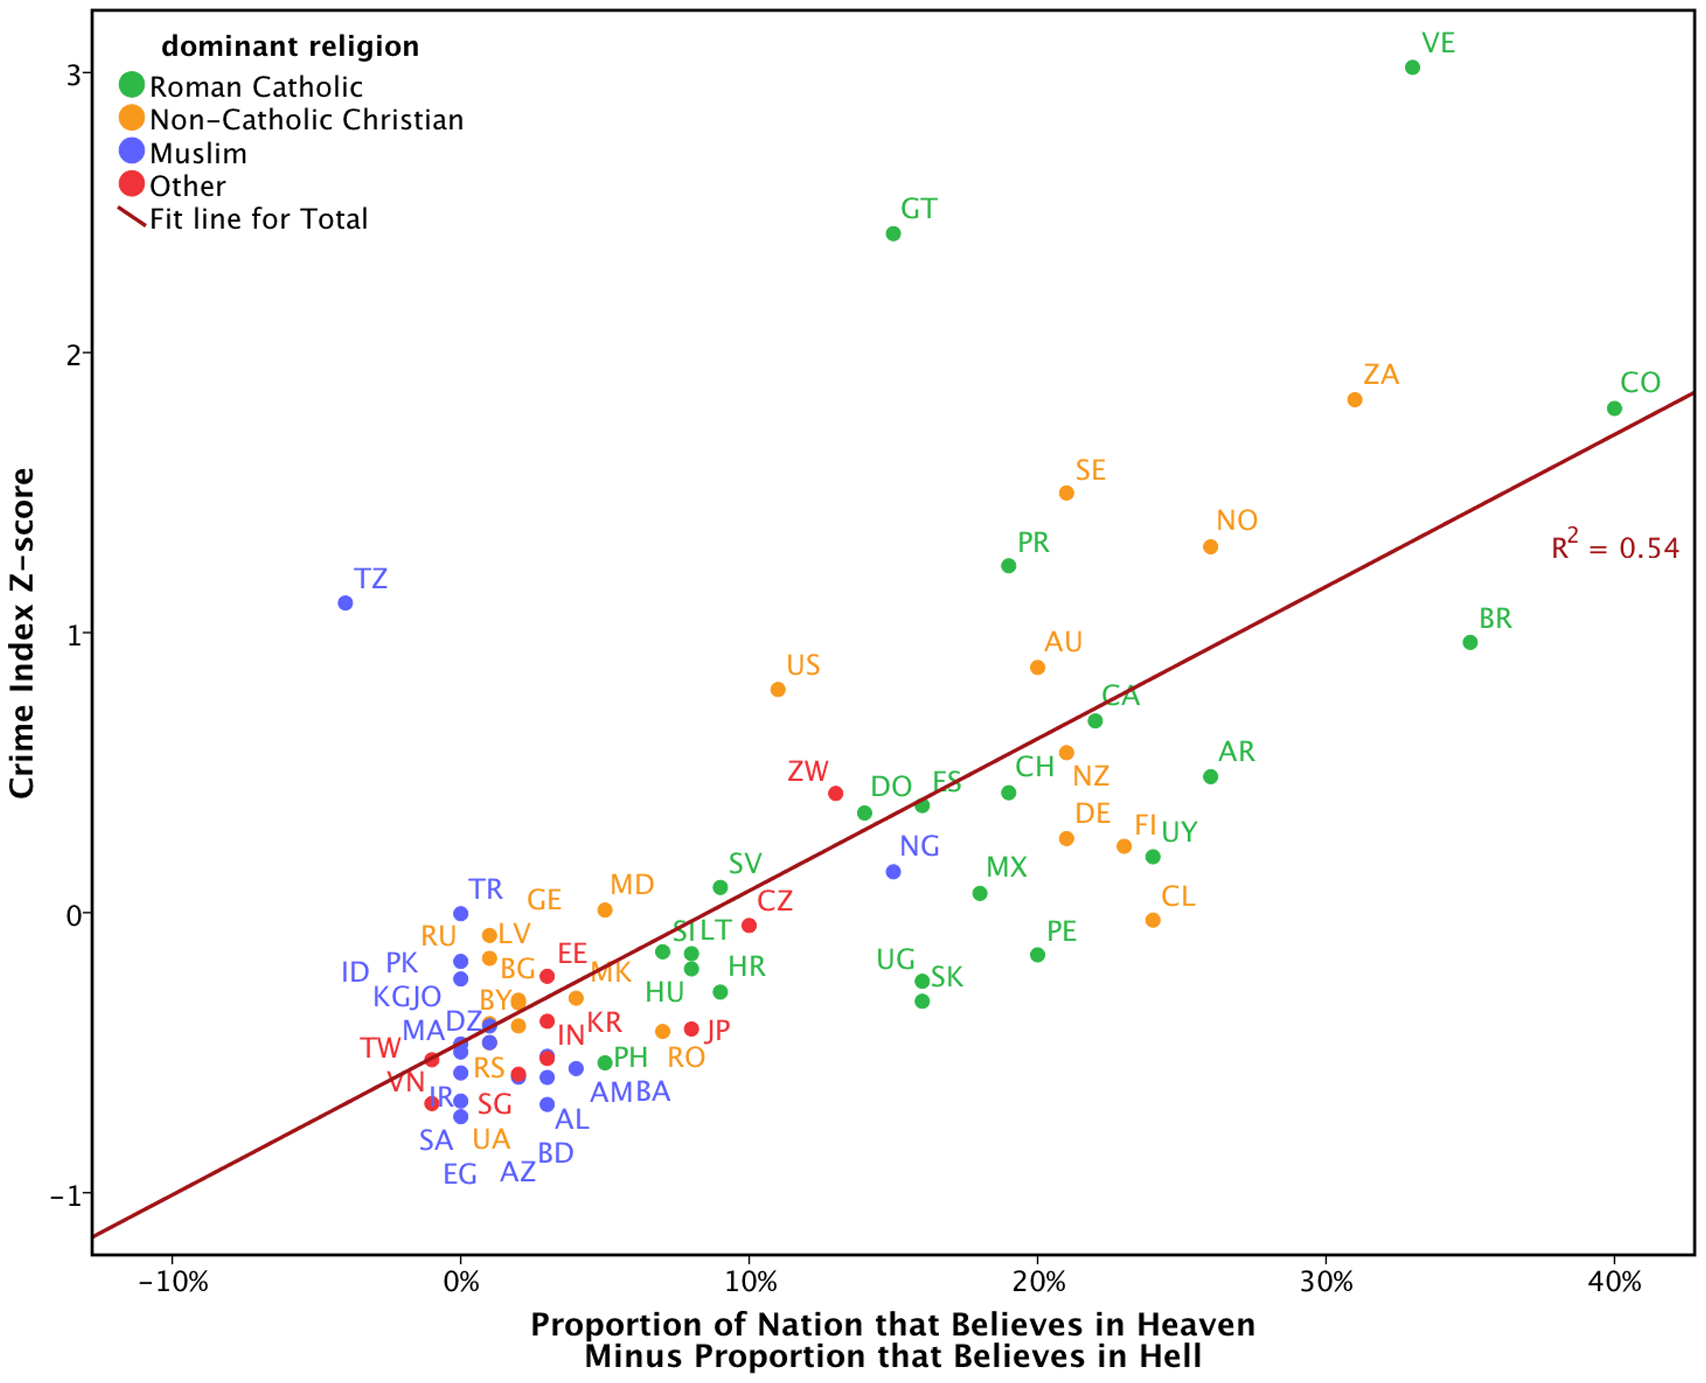
\includegraphics[width=0.7\textwidth]{images/hellvsheaven.png}}
    \end{figure}
\end{frame}

\begin{frame}[fragile]
    \frametitle{More Project Ideas}
    \begin{center}
    \href{http://www.stat.berkeley.edu/users/statlabs/}{http://www.stat.berkeley.edu/}
    \end{center}
    \vskip0.25in
    \begin{center}
        \href{http://www.math.msu.edu/Academic%5FPrograms/graduate/msim//ProjectPage.aspx}{http://www.math.msu.edu/}
    \end{center}
    \vskip0.25in
    \begin{center}
        \href{http://www.mathgoespop.com/2011/09/moneyball.html}{http://www.mathgoespop.com/}
    \end{center}
    \vskip0.25in
    \begin{center}
        \href{http://www.math.hmc.edu/clinic/projects/years/}{http://www.math.hmc.edu/clinic/}
    \end{center}
\end{frame}

\subsection{Insurance Redlining}


\newtheorem{DEFinsredlining}{Insurance Redlining}
\newtheorem{DEFfairplan}{FAIR}
\begin{frame}
    \frametitle{Example: Insurance Redlining}
    \begin{DEFinsredlining}
        \textcolor{red}{Insurance redlining} refers to the practice of refusing
        to issue insurance to certain types of people or within some 
        geographic area. 
    \end{DEFinsredlining}
\vskip.5in
    \begin{DEFfairplan}
        The \textcolor{red}{FAIR} plan was offered by the city of Chicago as a 
        default policy to homeowner who had been rejected by the voluntary
        market. 
    \end{DEFfairplan}
\end{frame}

\begin{frame}
    \frametitle{Example: Insurance Redlining}
    \begin{figure}
        \centering
        \caption{Insurance Redlining}
        \href{http://en.wikipedia.org/wiki/Redlining}{
        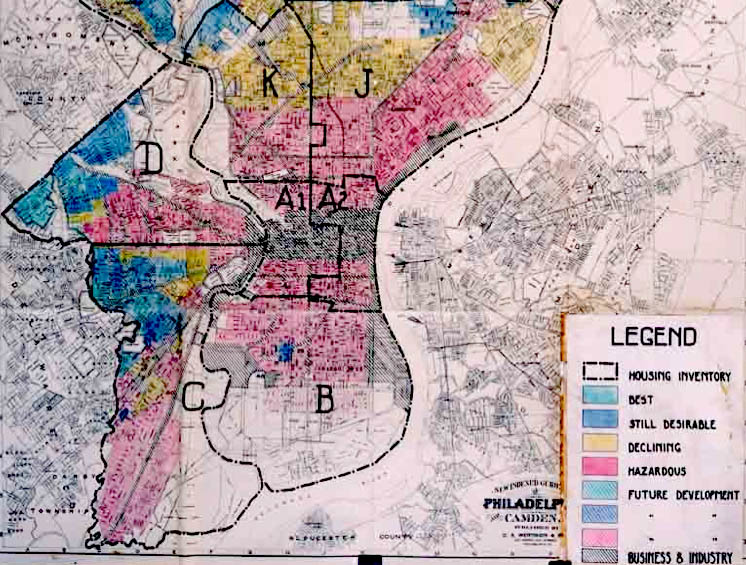
\includegraphics[width=0.8\textwidth]{redliningPhilly.jpg}
        }
                \label{fig:redlining}
    \end{figure}
\end{frame}



\newtheorem{DEFsponsorUSCCR}{Sponsor}
\newtheorem{DEFdataFAIR}{Data}
\begin{frame}
    \frametitle{Example: Insurance Redlining}
    \begin{DEFsponsorUSCCR} 
        The \href{http://www.usccr.gov/about/}{\textcolor{red}{U.S.~Commission
        on Civil Rights}} examined 
        charges by several Chicago community organizations that insurance 
        companies were redlining their neighborhoods. 
    \end{DEFsponsorUSCCR}
    \vskip.5in
    \begin{DEFdataFAIR}
        The \textcolor{red}{number of FAIR plan policies} written and renewed in Chicago
        by zip code for the number of months of December 1977 through May
        1978.
    \end{DEFdataFAIR}
\end{frame}

\begin{frame}
    \frametitle{Example: Insurance Redlining}
    Variables to consider:
    \begin{description}
        \item[\texttt{race}] Racial composition in percentage of minority,
        \item[\texttt{fire}] Fire per 100 housing units,
        \item[\texttt{theft}] Theft per 1000 population,
        \item[\texttt{age}] percent of housing unit built before 1939,
        \item[\texttt{involact}] New FAIR plan policies and renewal per 100 housing units,
        \item[\texttt{income}] Median family income in thousands of dollars,
        \item[\texttt{side}] North or South side of Chicago.
    \end{description}
\end{frame}

\newtheorem{DEFecofallacy}{Ecological Fallacy}
\begin{frame}
    \frametitle{Example: Ecological Fallacy}
    \begin{DEFecofallacy}
       When data are collected at the group level, we may observe 
       a correlation between two variables.  The \textcolor{red}{ecological
       fallacy} is concluding that the same correlation holds at the
       individual level. 
    \end{DEFecofallacy}
\end{frame}

\begin{frame}
    \frametitle{Example: Ecological Fallacy}
    \begin{figure}
        \centering
        \caption{1998 annual per capita income and proportion U.S.~born for 50
        states plus D.C.}
        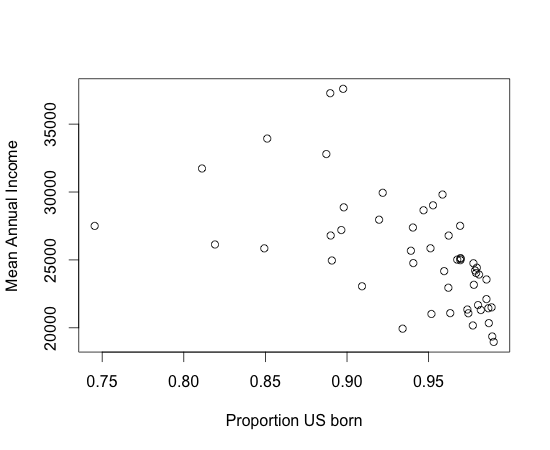
\includegraphics[width=0.75\textwidth]{images/FigureFarawayFigure11dot1.png}
    \end{figure}
\end{frame}

\begin{frame}
    \frametitle{Example: Ecological Fallacy}
    \begin{figure}
        \centering
        \caption{1998 annual per capita income and proportion U.S.~born for 50
        states plus D.C.}
        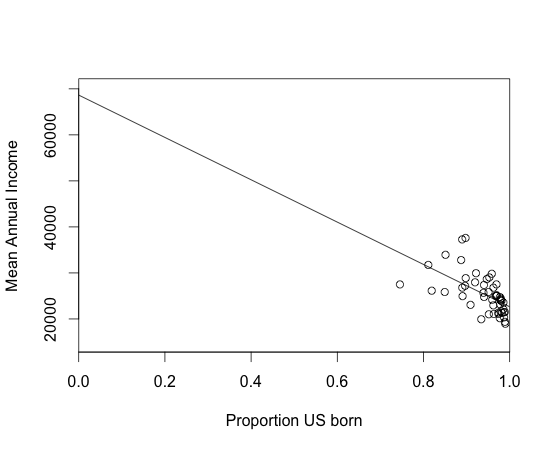
\includegraphics[width=0.75\textwidth]{images/FigureFarawayFigure11dot1b.png}
    \end{figure}
\end{frame}

\begin{frame}[fragile]
    \frametitle{Example: Insurance Redlining}
    \begin{verse}
For the ecological fallacy example, 
the assumption would be that the incomes of 
the native born do not depend on the proportion of native 
born within the state (and similarly for naturalized citizens).
    \end{verse}
    \vskip0.5in
    \begin{verse}
        For the insurance redlining example, we only have aggregate data.  
        We must inform the sponsor that unless more detailed data becomes
        available, the results for the aggregated data may not hold true 
        at the individual level. 
    \end{verse}
\end{frame}


\subsection{Sherlock Holmes and the Bicycle Tracks}

\begin{frame}
    \frametitle{Example: Sherlock Holmes and the Bicycle Tracks}
    \begin{verse}
        ``This track, as you perceive, was made by a rider who was going from
        the direction of the school.''
    \end{verse}
    \begin{verse}
        ``Or Toward it?''
    \end{verse}
    \begin{verse}
        ``No, no, my dear Watson.  The more deeply sunk impression is, of
        course, the hind wheel, upon which the weight rests.  You perceive
        several places where it has passed across and obliterated the more
        shallow mark of the front one.  It was undoubtedly heading away from
        the school.''
    \end{verse}
    \hfill -- \textit{The Adventure of the Priory School} by Arthur Conan Doyle
\end{frame}

\begin{frame}
    \frametitle{Example: Sherlock Holmes and the Bicycle Tracks}
    \begin{figure}
        \caption{Which one is the front wheel?}
        \begin{center}
            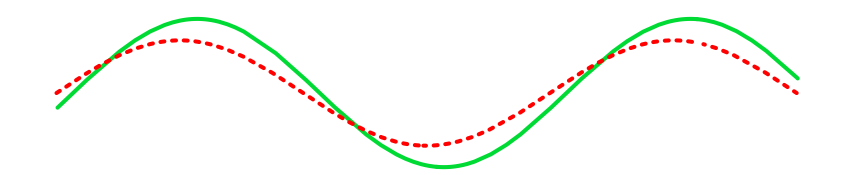
\includegraphics[width=\textwidth]{images/sholmesbike.png}
        \end{center}
        \label{fig:sholmesbike}
    \end{figure}
\end{frame}

\section{Tutorials}

\subsection{\LaTeX}

\begin{frame}
    \frametitle{Programmings in this class}
    \begin{itemize}
        \item \LaTeXs: 
            \begin{itemize}
                \item \texttt{moderncv}
                \item \texttt{beamer}
                \item \texttt{report}
                \item \href{http://www.texample.net}{\texttt{pgf/TikZ}}
            \end{itemize}
        \item Git
            \begin{itemize}
                \item \href{http://git-scm.com/doc}{\texttt{git gui}}
            \end{itemize}
        \item R:
            \begin{itemize}
                \item \texttt{lm}
                \item \href{https://catalyst.library.jhu.edu/catalog/bib_3642743}{\texttt{ggplot2}}
                \item \href{http://www.texample.net/tikz/examples/tikzdevice-demo/}{\texttt{tikzDevice}}
                \item \href{http://www.public.iastate.edu/~dicook/VIGRE/R-packages-slides.pdf}{\texttt{R CMD build}}
            \end{itemize}
    \end{itemize}
\end{frame}


\begin{frame}[fragile]
    \frametitle{Where to get some help for \LaTeXs}
    \begin{center}
    \href{http://en.wikibooks.org/wiki/LaTeX/}{http://en.wikibooks.org/wiki/LaTeX/}
    \end{center}
\end{frame}

\begin{frame}[fragile]
    \frametitle{Tutorial: \LaTeXs}
    \LaTeXs is a computer language for writing a scholarly paper:
    \begin{table}
        \centering
        \caption{HTML vs \LaTeXs}
        \begin{tabular}{c|p{3cm}|p{3cm}}
            \quad   &   HTML    & \LaTeXs \\ 
            \hline
            Code    & 
            \begin{lstlisting}
<html> 
 . . .
</html>
            \end{lstlisting} &  
            \begin{lstlisting}
\begin{document}
 . . .
\end{document}
            \end{lstlisting}\\
            \hline
            Compiler & Firefox and etc. & pdflatex and etc. \\
            \hline
            Output  & Web-page & PDF file
        \end{tabular}
        \label{tab:htmlvslatex}
    \end{table}
\end{frame}

\begin{frame}
    \frametitle{Tutorial: \LaTeXs}
    TeXworks is:
    \begin{itemize}
        \item an editing tool that is separate from \LaTeX,
        \item available in Linux, OSX and Windows,
        \item avaiable in: 
    \end{itemize}
    \vskip0.3in
    \begin{center}
    \href{http://code.google.com/p/texworks/}
    {http://code.google.com/p/texworks/}
    \end{center}
\end{frame}


\begin{frame}[fragile]
    \frametitle{Tutorial: \LaTeXs}
    \begin{itemize}
        \item Demo on preparing a resume using \LaTeXs \texttt{moderncv} package:
            \begin{itemize}
                \item Install \LaTeXs (MikTeX in Windows and MacTeX in OSX),
                \item Download \texttt{moderncv} package files from the course folder,
                \item Change file names to reflect you,
                \item Edit the TeX file,
                \item Compile using your favorite \LaTeXs editor,
                \item Look at the resulting PDF file.
            \end{itemize}
    \end{itemize}
\end{frame}

%\begin{frame}
%    \frametitle{Demo: \LaTeXs}
%    \begin{center}
%        \href{http://cdn.theladders.net/static/pdf/Senator_Obama_Resume.pdf}{In cObama's resume}
%    \end{center}
%\end{frame}

\begin{frame}[fragile]
    \frametitle{Cautions: \LaTeXs}
    There are numerous quirky \LaTeXs rules:
    \begin{itemize}
        \item opening quotation is not the same as the closing quotation,
        \item period yields \emph{two} blank spaces, 
        \item for \%, need to type \verb+\%+,
        \item for \textbackslash, need to type \verb+\textbackslash+,
        \item for /, need to type /,
        \item for \{, need to type \verb+\{+,
        \item for \$, need to type \verb+\$+,
        \item \verb+~+ yields a single blank space,
        \item and etc.
    \end{itemize}
\end{frame}


\subsection{Git}

\begin{frame}
    \frametitle{The place to get some Git helps}
    \begin{center}
        \href{http://git-scm.com/doc/}{http://git-scm.com/doc/}
    \end{center}
\end{frame}



\newtheorem{POEMbender}{The Blind Men and the Elephant}
\begin{frame}[fragile]
    \frametitle{Demo: \LaTeXs + Git}
    \begin{POEMbender}
    (HW for class activities)
    \end{POEMbender}
        \begin{itemize}
            \item Start up a git folder
            \item Create and edit the \texttt{.gitignore} file
            \item Download the template for a beamer file
            \item Look up the poem from the book
            \item One slide per stanza
            \item Compile after each stanza
            \item Commit after creating each stanza
            \item Repeat until done.
        \end{itemize}
\end{frame}

\begin{frame}[fragile]
    \frametitle{Tutorial: Git}

\begin{lstlisting}
sudo apt-get install git
\end{lstlisting}

\begin{figure}[b]
    \caption{An alternative: \texttt{git gui}}
    \begin{center}
        
\includegraphics[height=0.6\textheight]{gitguiinstall.png}
    \end{center}
    \label{fig:gitgui}
\end{figure}
    
\end{frame}

\begin{frame}[fragile]
    \frametitle{Tutorial: Git}

\vspace{8pt}
\begin{lstlisting}
cd ~/
git clone http://cis.jhu.edu/~nhlee/550400.git
\end{lstlisting}

\begin{figure}[b]
    \caption{An alternative: \texttt{git gui}}
    \begin{center}
        
\includegraphics[height=0.5\textheight]{gitgui.png}
    \end{center}
    \label{fig:gitgui2}
\end{figure}
    
\end{frame}

\begin{frame}[fragile]
    \frametitle{Tutorial: Git}
\begin{lstlisting}
cd ~/550400
git reset --hard HEAD
git pull origin master
\end{lstlisting}
\begin{figure}[b]
    \centering
    \caption{An alternative: \texttt{git gui}}
        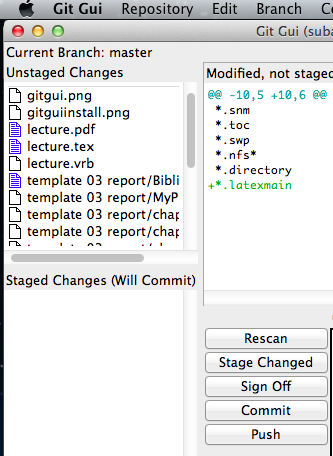
\includegraphics[height=0.6\textheight]{gitguiusing.png}
    \label{fig:gitgui4}
\end{figure}
\end{frame}



\begin{frame}[fragile]
    \frametitle{Tutorial: Git}
    After years of using git, you might find this funny: 
    \begin{columns}
        \begin{column}{0.5\textwidth}
            \begin{figure}
                \begin{center}
                    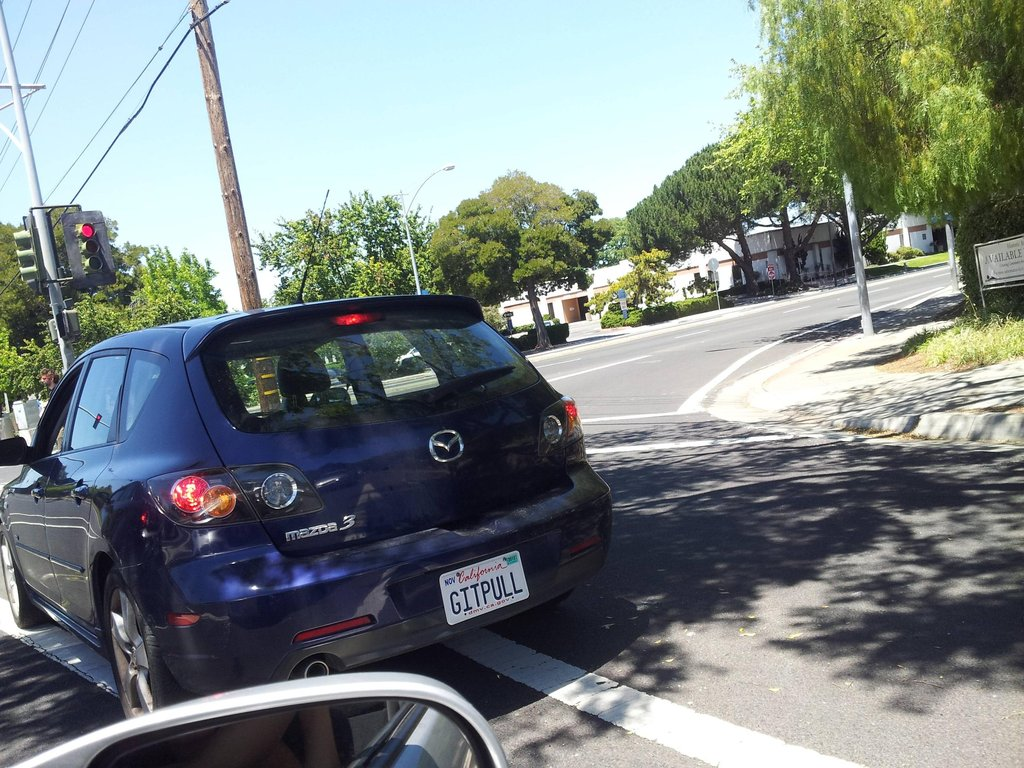
\includegraphics[width=\textwidth]{images/gitpull.jpg}
                \end{center}
            \end{figure}
        \end{column}
        \begin{column}{0.5\textwidth}
            \begin{lstlisting}
git pull origin master
            \end{lstlisting}
        \end{column}
    \end{columns} 
\end{frame}

\begin{frame}[fragile]
    \frametitle{Tutorial: Git}
    After years of using git, you might find this funny: 
    \begin{columns}
        \begin{column}{0.5\textwidth}
            \begin{figure}
                \begin{center}
                    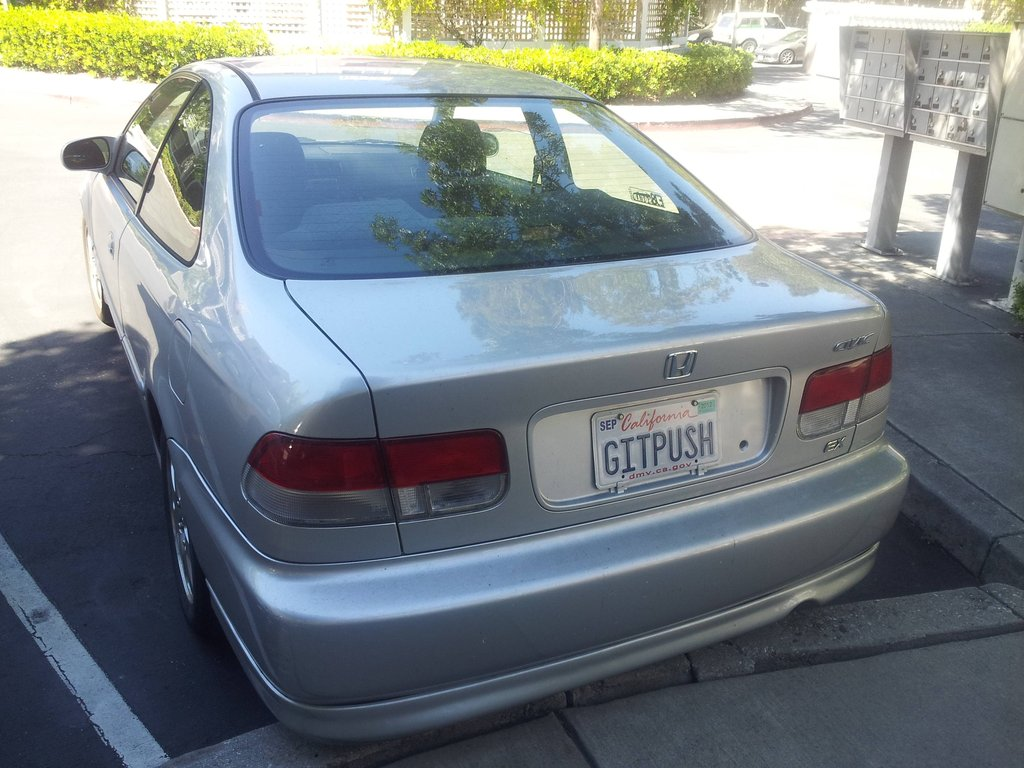
\includegraphics[width=\textwidth]{images/gitpush.jpg}
                \end{center}
            \end{figure}
        \end{column}
        \begin{column}{0.5\textwidth}
            \begin{lstlisting}
git push origin master
            \end{lstlisting}
        \end{column}
    \end{columns} 
\end{frame}

\begin{frame}[fragile]
    \frametitle{Tutorial: Git}
    \begin{columns}
        \begin{column}{0.4\textwidth}
            \begin{figure}
                \caption{For \$19.99, you can also have your own:}
                \begin{center}
                    
\includegraphics[width=\textwidth]{images/gitrdone.jpg}
                \end{center}
            \end{figure}
        \end{column}
        \begin{column}{0.6\textwidth}
\begin{lstlisting}
cd ~/
mkdir hub.git
mkdir computerA.git
mkdir computerB.git

git init --bare hub.git

cd hub.git
cd hooks
cp post-update.sample post-update
\end{lstlisting}
        \end{column}
    \end{columns} 
\end{frame}

\begin{frame}[fragile]
    \frametitle{Tutorial: Git}
    \begin{columns}
        \begin{column}{0.5\textwidth}
\begin{lstlisting}
cd computerA.git
git init 
git remote add origin ~/hub.git
cat Hello >> commonfile.txt
git add commonfile.txt 
git pull origin master
git commit -am 'from A'
git push origin master
\end{lstlisting}
        \end{column}
        \begin{column}{0.5\textwidth}
\begin{lstlisting}
cd computerB.git
git init 
git remote add origin ~/hub.git
cat World >> fileB.txt
git add commonfile.txt 
git pull origin master
git commit -am 'from B'
git push origin master
\end{lstlisting}
        \end{column}
    \end{columns} 
\end{frame}


\begin{frame}[fragile]
    \frametitle{Tutorial: Git}
    \begin{columns}
        \begin{column}{0.5\textwidth}
    \begin{lstlisting}
cd ~/550400

git status 
git add .
git commit -am 'done now'

git branch personal
git branch
git checkout personal

edit some file 
git status 
git add . 
git commit -am 'personal edit'

git checkout master
git branch -D personal
    \end{lstlisting}
        \end{column}
        \begin{column}{0.5\textwidth}
    \begin{itemize}
        \item checks if there has been any change to the folder
        \item build and update the \texttt{master} git branch
        \item create and update a \texttt{personal} git branch
    \end{itemize}
        \end{column}
    \end{columns} 
\end{frame}



\begin{frame}
    \frametitle{Tutorial: Git}
    \texttt{.gitignore}?
    \vskip0.1in
    \begin{itemize}
        \item N.B.~the course folder already has one 
        \item Use it to let \emph{git} know the files to \emph{ignore} while
            version controlling
        \item one particular usage: create \texttt{.gitignore} at the root of
            your git folder 
        \item files already been list under the git watch list will not be
            ignored even after creation of \texttt{.gitignore} 
    \end{itemize}
\end{frame}

\subsection{Vim}
\begin{frame}
    \frametitle{Vim}
    \begin{center}
        Vim is a \emph{highly customizable} text editor 
    \end{center}
\end{frame}

\subsection{R}

\begin{frame}[fragile]
    \frametitle{Demo: R + \LaTeX}
    \begin{columns}
        \begin{column}{0.5\textwidth}
            \begin{figure}
                \centering
            \caption{R Studio}
            \href{http://rstudio.org}{
            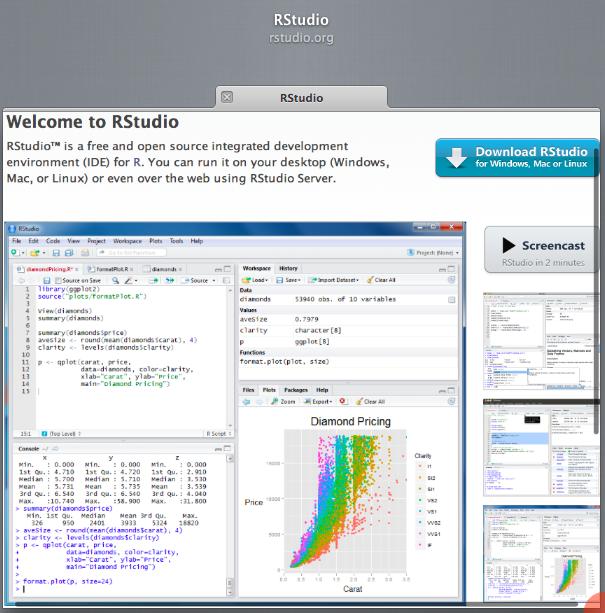
\includegraphics[width=\textwidth]{images/Rstudio}
            }
        \end{figure}
        \end{column}
        \begin{column}{0.5\textwidth}
            \begin{figure}
                \centering
                        \caption{R}
                    \href{http://www.r-project.org}{
                        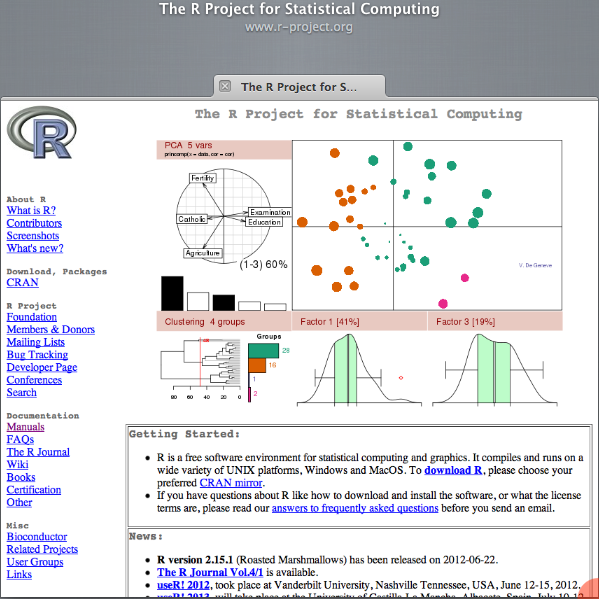
\includegraphics[width=\textwidth]{images/Rproject}}
            \end{figure}
        \end{column}
    \end{columns} 
\end{frame}

\begin{frame}[fragile]
    \frametitle{Demo: R + \LaTeX}
    \begin{columns}
        \begin{column}{0.45\textwidth}
    \begin{lstlisting}
install.packages(faraway)
install.packages(tikzDevice)
require(faraway)
require(tikzDevice)
data(eco)
tikz('embeddedfig1.tex', 
    standAlone=F, 
    width=5,height=5)
plot(income ~ usborn, 
    data=eco,
    xlab=`Proportion US born'
    ylab=`Mean Annual Income'
    )
dev.off()
    \end{lstlisting}
        \end{column}
        \begin{column}{0.55\textwidth}
        \begin{figure}[0.8\textwidth]
            % Created by tikzDevice version 0.6.2 on 2012-09-11 12:28:03
% !TEX encoding = UTF-8 Unicode
\begin{tikzpicture}[x=1pt,y=1pt,scale=0.5]
\definecolor[named]{drawColor}{rgb}{0.00,0.00,0.00}
\definecolor[named]{fillColor}{rgb}{1.00,1.00,1.00}
\fill[color=fillColor,fill opacity=0.00,] (0,0) rectangle (361.35,361.35);
\begin{scope}
\path[clip] ( 49.20, 61.20) rectangle (336.15,312.15);
\definecolor[named]{fillColor}{rgb}{0.00,0.00,0.00}
\definecolor[named]{drawColor}{rgb}{0.00,0.00,0.00}

\draw[color=drawColor,line cap=round,line join=round,fill opacity=0.00,] (321.92,101.46) circle (  2.25);

\draw[color=drawColor,line cap=round,line join=round,fill opacity=0.00,] (270.39,154.23) circle (  2.25);

\draw[color=drawColor,line cap=round,line join=round,fill opacity=0.00,] (237.82,121.63) circle (  2.25);

\draw[color=drawColor,line cap=round,line join=round,fill opacity=0.00,] (322.27, 87.80) circle (  2.25);

\draw[color=drawColor,line cap=round,line join=round,fill opacity=0.00,] ( 59.83,177.01) circle (  2.25);

\draw[color=drawColor,line cap=round,line join=round,fill opacity=0.00,] (278.80,191.40) circle (  2.25);

\draw[color=drawColor,line cap=round,line join=round,fill opacity=0.00,] (225.25,302.86) circle (  2.25);

\draw[color=drawColor,line cap=round,line join=round,fill opacity=0.00,] (291.43,205.82) circle (  2.25);

\draw[color=drawColor,line cap=round,line join=round,fill opacity=0.00,] (216.67,298.87) circle (  2.25);

\draw[color=drawColor,line cap=round,line join=round,fill opacity=0.00,] (172.76,156.43) circle (  2.25);

\draw[color=drawColor,line cap=round,line join=round,fill opacity=0.00,] (301.22,146.06) circle (  2.25);

\draw[color=drawColor,line cap=round,line join=round,fill opacity=0.00,] (139.93,159.99) circle (  2.25);

\draw[color=drawColor,line cap=round,line join=round,fill opacity=0.00,] (296.56, 96.96) circle (  2.25);

\draw[color=drawColor,line cap=round,line join=round,fill opacity=0.00,] (225.68,194.09) circle (  2.25);

\draw[color=drawColor,line cap=round,line join=round,fill opacity=0.00,] (313.14,136.08) circle (  2.25);

\draw[color=drawColor,line cap=round,line join=round,fill opacity=0.00,] (315.76,132.41) circle (  2.25);

\draw[color=drawColor,line cap=round,line join=round,fill opacity=0.00,] (303.32,145.58) circle (  2.25);

\draw[color=drawColor,line cap=round,line join=round,fill opacity=0.00,] (324.10,102.26) circle (  2.25);

\draw[color=drawColor,line cap=round,line join=round,fill opacity=0.00,] (307.96,100.26) circle (  2.25);

\draw[color=drawColor,line cap=round,line join=round,fill opacity=0.00,] (295.32,120.28) circle (  2.25);

\draw[color=drawColor,line cap=round,line join=round,fill opacity=0.00,] (251.62,207.43) circle (  2.25);

\draw[color=drawColor,line cap=round,line join=round,fill opacity=0.00,] (214.06,243.01) circle (  2.25);

\draw[color=drawColor,line cap=round,line join=round,fill opacity=0.00,] (283.42,156.50) circle (  2.25);

\draw[color=drawColor,line cap=round,line join=round,fill opacity=0.00,] (303.14,177.10) circle (  2.25);

\draw[color=drawColor,line cap=round,line join=round,fill opacity=0.00,] (325.52, 70.49) circle (  2.25);

\draw[color=drawColor,line cap=round,line join=round,fill opacity=0.00,] (314.27,138.67) circle (  2.25);

\draw[color=drawColor,line cap=round,line join=round,fill opacity=0.00,] (311.62, 85.63) circle (  2.25);

\draw[color=drawColor,line cap=round,line join=round,fill opacity=0.00,] (312.00,142.75) circle (  2.25);

\draw[color=drawColor,line cap=round,line join=round,fill opacity=0.00,] (224.04,173.24) circle (  2.25);

\draw[color=drawColor,line cap=round,line join=round,fill opacity=0.00,] (285.10,195.95) circle (  2.25);

\draw[color=drawColor,line cap=round,line join=round,fill opacity=0.00,] (174.71,257.22) circle (  2.25);

\draw[color=drawColor,line cap=round,line join=round,fill opacity=0.00,] (264.86, 82.69) circle (  2.25);

\draw[color=drawColor,line cap=round,line join=round,fill opacity=0.00,] (131.29,229.76) circle (  2.25);

\draw[color=drawColor,line cap=round,line join=round,fill opacity=0.00,] (313.79,133.80) circle (  2.25);

\draw[color=drawColor,line cap=round,line join=round,fill opacity=0.00,] (315.08,104.36) circle (  2.25);

\draw[color=drawColor,line cap=round,line join=round,fill opacity=0.00,] (303.42,147.48) circle (  2.25);

\draw[color=drawColor,line cap=round,line join=round,fill opacity=0.00,] (308.62, 96.85) circle (  2.25);

\draw[color=drawColor,line cap=round,line join=round,fill opacity=0.00,] (271.97,142.90) circle (  2.25);

\draw[color=drawColor,line cap=round,line join=round,fill opacity=0.00,] (295.52,168.15) circle (  2.25);

\draw[color=drawColor,line cap=round,line join=round,fill opacity=0.00,] (216.98,168.21) circle (  2.25);

\draw[color=drawColor,line cap=round,line join=round,fill opacity=0.00,] (316.94, 99.80) circle (  2.25);

\draw[color=drawColor,line cap=round,line join=round,fill opacity=0.00,] (320.67,109.84) circle (  2.25);

\draw[color=drawColor,line cap=round,line join=round,fill opacity=0.00,] (320.71,127.85) circle (  2.25);

\draw[color=drawColor,line cap=round,line join=round,fill opacity=0.00,] (217.76,145.28) circle (  2.25);

\draw[color=drawColor,line cap=round,line join=round,fill opacity=0.00,] (284.06, 96.19) circle (  2.25);

\draw[color=drawColor,line cap=round,line join=round,fill opacity=0.00,] (292.53,135.53) circle (  2.25);

\draw[color=drawColor,line cap=round,line join=round,fill opacity=0.00,] (271.72,175.54) circle (  2.25);

\draw[color=drawColor,line cap=round,line join=round,fill opacity=0.00,] (249.19,182.72) circle (  2.25);

\draw[color=drawColor,line cap=round,line join=round,fill opacity=0.00,] (324.52, 75.53) circle (  2.25);

\draw[color=drawColor,line cap=round,line join=round,fill opacity=0.00,] (303.47,146.80) circle (  2.25);

\draw[color=drawColor,line cap=round,line join=round,fill opacity=0.00,] (312.30,122.96) circle (  2.25);
\end{scope}
\begin{scope}
\path[clip] (  0.00,  0.00) rectangle (361.35,361.35);
\definecolor[named]{fillColor}{rgb}{0.00,0.00,0.00}
\definecolor[named]{drawColor}{rgb}{0.00,0.00,0.00}

\draw[color=drawColor,line cap=round,line join=round,fill opacity=0.00,] ( 64.82, 61.20) -- (282.19, 61.20);

\draw[color=drawColor,line cap=round,line join=round,fill opacity=0.00,] ( 64.82, 61.20) -- ( 64.82, 55.20);

\draw[color=drawColor,line cap=round,line join=round,fill opacity=0.00,] (119.16, 61.20) -- (119.16, 55.20);

\draw[color=drawColor,line cap=round,line join=round,fill opacity=0.00,] (173.50, 61.20) -- (173.50, 55.20);

\draw[color=drawColor,line cap=round,line join=round,fill opacity=0.00,] (227.85, 61.20) -- (227.85, 55.20);

\draw[color=drawColor,line cap=round,line join=round,fill opacity=0.00,] (282.19, 61.20) -- (282.19, 55.20);

\node[color=drawColor,anchor=base,inner sep=0pt, outer sep=0pt, scale=  1.00] at ( 64.82, 37.20) {\tiny 0.75};
\node[color=drawColor,anchor=base,inner sep=0pt, outer sep=0pt, scale=  1.00] at (119.16, 37.20) {\tiny 0.80};
\node[color=drawColor,anchor=base,inner sep=0pt, outer sep=0pt, scale=  1.00] at (173.50, 37.20) {\tiny 0.85};
\node[color=drawColor,anchor=base,inner sep=0pt, outer sep=0pt, scale=  1.00] at (227.85, 37.20) {\tiny 0.90};
\node[color=drawColor,anchor=base,inner sep=0pt, outer sep=0pt, scale=  1.00] at (282.19, 37.20) {\tiny 0.95};

\draw[color=drawColor,line cap=round,line join=round,fill opacity=0.00,] ( 49.20, 83.48) -- ( 49.20,270.47);

\draw[color=drawColor,line cap=round,line join=round,fill opacity=0.00,] ( 49.20, 83.48) -- ( 43.20, 83.48);

\draw[color=drawColor,line cap=round,line join=round,fill opacity=0.00,] ( 49.20,145.81) -- ( 43.20,145.81);

\draw[color=drawColor,line cap=round,line join=round,fill opacity=0.00,] ( 49.20,208.14) -- ( 43.20,208.14);

\draw[color=drawColor,line cap=round,line join=round,fill opacity=0.00,] ( 49.20,270.47) -- ( 43.20,270.47);

\node[rotate= 90.00,color=drawColor,anchor=base,inner sep=0pt, outer sep=0pt,
scale=  1.00] at ( 37.20, 83.48) {\tiny 20000};

\node[rotate= 90.00,color=drawColor,anchor=base,inner sep=0pt, outer sep=0pt,
scale=  1.00] at ( 37.20,145.81) {\tiny 25000};

\node[rotate= 90.00,color=drawColor,anchor=base,inner sep=0pt, outer sep=0pt,
scale=  1.00] at ( 37.20,208.14) {\tiny 30000};

\node[rotate= 90.00,color=drawColor,anchor=base,inner sep=0pt, outer sep=0pt,
scale=  1.00] at ( 37.20,270.47) {\tiny 35000};

\draw[color=drawColor,line cap=round,line join=round,fill opacity=0.00,] ( 49.20, 61.20) --
	(336.15, 61.20) --
	(336.15,312.15) --
	( 49.20,312.15) --
	( 49.20, 61.20);
\end{scope}
\begin{scope}
\path[clip] (  0.00,  0.00) rectangle (361.35,361.35);
\definecolor[named]{fillColor}{rgb}{0.00,0.00,0.00}
\definecolor[named]{drawColor}{rgb}{0.00,0.00,0.00}

\node[color=drawColor,anchor=base,inner sep=0pt, outer sep=0pt, scale=  1.00]
at (192.67, 13.20) {USborn};

\node[rotate= 90.00,color=drawColor,anchor=base,inner sep=0pt, outer sep=0pt,
scale=  1.00] at ( 13.20,186.67) {Income};
\end{scope}
\end{tikzpicture}

        \end{figure}
        \end{column}
    \end{columns} 
\end{frame}

\begin{frame}[fragile]
    \frametitle{Demo: R + \LaTeX}
    \begin{columns}
        \begin{column}{0.45\textwidth}
            \begin{lstlisting}
tikz('embeddedfig2.tex', 
    standAlone=F, 
    width=5,height=5)
plot(income ~ usborn, 
    data = eco,
    xlab=`Proportion US born',
    ylab=`Mean Annual Income',
    xlim=c(0,1),
    ylim=c(15000,70000),
    xaxs='i')
g<-lm(income~usborn,eco)
abline(coef(g))
dev.off()
            \end{lstlisting}
        \end{column}
        \begin{column}{0.55\textwidth}
            % Created by tikzDevice version 0.6.2 on 2012-09-11 13:10:12
% !TEX encoding = UTF-8 Unicode
\begin{tikzpicture}[x=1pt,y=1pt,scale=0.5]
\definecolor[named]{drawColor}{rgb}{0.00,0.00,0.00}
\definecolor[named]{fillColor}{rgb}{1.00,1.00,1.00}
\fill[color=fillColor,fill opacity=0.00,] (0,0) rectangle (361.35,361.35);
\begin{scope}
\path[clip] ( 49.20, 61.20) rectangle (336.15,312.15);
\definecolor[named]{drawColor}{rgb}{0.00,0.00,0.00}

\draw[color=drawColor,line cap=round,line join=round,fill opacity=0.00,] (332.29, 97.71) circle (  2.25);

\draw[color=drawColor,line cap=round,line join=round,fill opacity=0.00,] (318.69,115.59) circle (  2.25);

\draw[color=drawColor,line cap=round,line join=round,fill opacity=0.00,] (310.09,104.55) circle (  2.25);

\draw[color=drawColor,line cap=round,line join=round,fill opacity=0.00,] (332.39, 93.08) circle (  2.25);

\draw[color=drawColor,line cap=round,line join=round,fill opacity=0.00,] (263.10,123.32) circle (  2.25);

\draw[color=drawColor,line cap=round,line join=round,fill opacity=0.00,] (320.91,128.19) circle (  2.25);

\draw[color=drawColor,line cap=round,line join=round,fill opacity=0.00,] (306.77,165.97) circle (  2.25);

\draw[color=drawColor,line cap=round,line join=round,fill opacity=0.00,] (324.24,133.08) circle (  2.25);

\draw[color=drawColor,line cap=round,line join=round,fill opacity=0.00,] (304.51,164.61) circle (  2.25);

\draw[color=drawColor,line cap=round,line join=round,fill opacity=0.00,] (292.91,116.34) circle (  2.25);

\draw[color=drawColor,line cap=round,line join=round,fill opacity=0.00,] (326.83,112.83) circle (  2.25);

\draw[color=drawColor,line cap=round,line join=round,fill opacity=0.00,] (284.24,117.55) circle (  2.25);

\draw[color=drawColor,line cap=round,line join=round,fill opacity=0.00,] (325.60, 96.19) circle (  2.25);

\draw[color=drawColor,line cap=round,line join=round,fill opacity=0.00,] (306.88,129.10) circle (  2.25);

\draw[color=drawColor,line cap=round,line join=round,fill opacity=0.00,] (329.97,109.44) circle (  2.25);

\draw[color=drawColor,line cap=round,line join=round,fill opacity=0.00,] (330.67,108.20) circle (  2.25);

\draw[color=drawColor,line cap=round,line join=round,fill opacity=0.00,] (327.38,112.66) circle (  2.25);

\draw[color=drawColor,line cap=round,line join=round,fill opacity=0.00,] (332.87, 97.98) circle (  2.25);

\draw[color=drawColor,line cap=round,line join=round,fill opacity=0.00,] (328.61, 97.30) circle (  2.25);

\draw[color=drawColor,line cap=round,line join=round,fill opacity=0.00,] (325.27,104.09) circle (  2.25);

\draw[color=drawColor,line cap=round,line join=round,fill opacity=0.00,] (313.73,133.62) circle (  2.25);

\draw[color=drawColor,line cap=round,line join=round,fill opacity=0.00,] (303.82,145.68) circle (  2.25);

\draw[color=drawColor,line cap=round,line join=round,fill opacity=0.00,] (322.13,116.36) circle (  2.25);

\draw[color=drawColor,line cap=round,line join=round,fill opacity=0.00,] (327.33,123.35) circle (  2.25);

\draw[color=drawColor,line cap=round,line join=round,fill opacity=0.00,] (333.24, 87.22) circle (  2.25);

\draw[color=drawColor,line cap=round,line join=round,fill opacity=0.00,] (330.27,110.32) circle (  2.25);

\draw[color=drawColor,line cap=round,line join=round,fill opacity=0.00,] (329.57, 92.34) circle (  2.25);

\draw[color=drawColor,line cap=round,line join=round,fill opacity=0.00,] (329.67,111.70) circle (  2.25);

\draw[color=drawColor,line cap=round,line join=round,fill opacity=0.00,] (306.45,122.04) circle (  2.25);

\draw[color=drawColor,line cap=round,line join=round,fill opacity=0.00,] (322.57,129.73) circle (  2.25);

\draw[color=drawColor,line cap=round,line join=round,fill opacity=0.00,] (293.43,150.50) circle (  2.25);

\draw[color=drawColor,line cap=round,line join=round,fill opacity=0.00,] (317.23, 91.35) circle (  2.25);

\draw[color=drawColor,line cap=round,line join=round,fill opacity=0.00,] (281.96,141.19) circle (  2.25);

\draw[color=drawColor,line cap=round,line join=round,fill opacity=0.00,] (330.15,108.67) circle (  2.25);

\draw[color=drawColor,line cap=round,line join=round,fill opacity=0.00,] (330.49, 98.69) circle (  2.25);

\draw[color=drawColor,line cap=round,line join=round,fill opacity=0.00,] (327.41,113.31) circle (  2.25);

\draw[color=drawColor,line cap=round,line join=round,fill opacity=0.00,] (328.78, 96.15) circle (  2.25);

\draw[color=drawColor,line cap=round,line join=round,fill opacity=0.00,] (319.11,111.75) circle (  2.25);

\draw[color=drawColor,line cap=round,line join=round,fill opacity=0.00,] (325.32,120.31) circle (  2.25);

\draw[color=drawColor,line cap=round,line join=round,fill opacity=0.00,] (304.59,120.33) circle (  2.25);

\draw[color=drawColor,line cap=round,line join=round,fill opacity=0.00,] (330.98, 97.15) circle (  2.25);

\draw[color=drawColor,line cap=round,line join=round,fill opacity=0.00,] (331.96,100.55) circle (  2.25);

\draw[color=drawColor,line cap=round,line join=round,fill opacity=0.00,] (331.97,106.65) circle (  2.25);

\draw[color=drawColor,line cap=round,line join=round,fill opacity=0.00,] (304.79,112.56) circle (  2.25);

\draw[color=drawColor,line cap=round,line join=round,fill opacity=0.00,] (322.30, 95.92) circle (  2.25);

\draw[color=drawColor,line cap=round,line join=round,fill opacity=0.00,] (324.53,109.26) circle (  2.25);

\draw[color=drawColor,line cap=round,line join=round,fill opacity=0.00,] (319.04,122.82) circle (  2.25);

\draw[color=drawColor,line cap=round,line join=round,fill opacity=0.00,] (313.09,125.25) circle (  2.25);

\draw[color=drawColor,line cap=round,line join=round,fill opacity=0.00,] (332.98, 88.92) circle (  2.25);

\draw[color=drawColor,line cap=round,line join=round,fill opacity=0.00,] (327.42,113.08) circle (  2.25);

\draw[color=drawColor,line cap=round,line join=round,fill opacity=0.00,] (329.75,105.00) circle (  2.25);
\end{scope}
\begin{scope}
\path[clip] (  0.00,  0.00) rectangle (361.35,361.35);
\definecolor[named]{drawColor}{rgb}{0.00,0.00,0.00}

\draw[color=drawColor,line cap=round,line join=round,fill opacity=0.00,] ( 49.20, 61.20) -- (336.15, 61.20);

\draw[color=drawColor,line cap=round,line join=round,fill opacity=0.00,] ( 49.20, 61.20) -- ( 49.20, 55.20);

\draw[color=drawColor,line cap=round,line join=round,fill opacity=0.00,] (106.59, 61.20) -- (106.59, 55.20);

\draw[color=drawColor,line cap=round,line join=round,fill opacity=0.00,] (163.98, 61.20) -- (163.98, 55.20);

\draw[color=drawColor,line cap=round,line join=round,fill opacity=0.00,] (221.37, 61.20) -- (221.37, 55.20);

\draw[color=drawColor,line cap=round,line join=round,fill opacity=0.00,] (278.76, 61.20) -- (278.76, 55.20);

\draw[color=drawColor,line cap=round,line join=round,fill opacity=0.00,] (336.15, 61.20) -- (336.15, 55.20);

\node[color=drawColor,anchor=base,inner sep=0pt, outer sep=0pt, scale=  1.00]
at ( 49.20, 37.20) {\tiny 0.0};

\node[color=drawColor,anchor=base,inner sep=0pt, outer sep=0pt, scale=  1.00] at (106.59, 37.20) {\tiny 0.2};

\node[color=drawColor,anchor=base,inner sep=0pt, outer sep=0pt, scale=  1.00] at (163.98, 37.20) {\tiny 0.4};

\node[color=drawColor,anchor=base,inner sep=0pt, outer sep=0pt, scale=  1.00] at (221.37, 37.20) {\tiny 0.6};

\node[color=drawColor,anchor=base,inner sep=0pt, outer sep=0pt, scale=  1.00] at (278.76, 37.20) {\tiny 0.8};

\node[color=drawColor,anchor=base,inner sep=0pt, outer sep=0pt, scale=  1.00] at (336.15, 37.20) {\tiny 1.0};

\draw[color=drawColor,line cap=round,line join=round,fill opacity=0.00,] ( 49.20, 91.62) -- ( 49.20,302.86);

\draw[color=drawColor,line cap=round,line join=round,fill opacity=0.00,] ( 49.20, 91.62) -- ( 43.20, 91.62);

\draw[color=drawColor,line cap=round,line join=round,fill opacity=0.00,] ( 49.20,133.87) -- ( 43.20,133.87);

\draw[color=drawColor,line cap=round,line join=round,fill opacity=0.00,] ( 49.20,176.11) -- ( 43.20,176.11);

\draw[color=drawColor,line cap=round,line join=round,fill opacity=0.00,] ( 49.20,218.36) -- ( 43.20,218.36);

\draw[color=drawColor,line cap=round,line join=round,fill opacity=0.00,] ( 49.20,260.61) -- ( 43.20,260.61);

\draw[color=drawColor,line cap=round,line join=round,fill opacity=0.00,] ( 49.20,302.86) -- ( 43.20,302.86);

\node[rotate= 90.00,color=drawColor,anchor=base,inner sep=0pt, outer sep=0pt,
scale=  1.00] at ( 37.20, 91.62) {\tiny 20000};

\node[rotate= 90.00,color=drawColor,anchor=base,inner sep=0pt, outer sep=0pt, scale=  1.00] at ( 37.20,133.87) {\tiny 30000};
\node[rotate= 90.00,color=drawColor,anchor=base,inner sep=0pt, outer sep=0pt, scale=  1.00] at ( 37.20,176.11) {\tiny 40000};
\node[rotate= 90.00,color=drawColor,anchor=base,inner sep=0pt, outer sep=0pt, scale=  1.00] at ( 37.20,218.36) {\tiny 50000};
\node[rotate= 90.00,color=drawColor,anchor=base,inner sep=0pt, outer sep=0pt, scale=  1.00] at ( 37.20,260.61) {\tiny 60000};
\node[rotate= 90.00,color=drawColor,anchor=base,inner sep=0pt, outer sep=0pt, scale=  1.00] at ( 37.20,302.86) {\tiny 70000};

\draw[color=drawColor,line cap=round,line join=round,fill opacity=0.00,] 
    ( 49.20, 61.20) --
	(336.15, 61.20) --
	(336.15,312.15) --
	( 49.20,312.15) --
	( 49.20, 61.20);
\end{scope}
\begin{scope}
\path[clip] (  0.00,  0.00) rectangle (361.35,361.35);
\definecolor[named]{drawColor}{rgb}{0.00,0.00,0.00}

\node[color=drawColor,anchor=base,inner sep=0pt, outer sep=0pt, scale=  1.00] at (192.68, 13.20) {Proportion US born};

\node[rotate= 90.00,color=drawColor,anchor=base,inner sep=0pt, outer sep=0pt, scale=  1.00] at ( 13.20,186.67) {Mean Annual Income};
\end{scope}
\begin{scope}
\path[clip] ( 49.20, 61.20) rectangle (336.15,312.15);
\definecolor[named]{drawColor}{rgb}{0.00,0.00,0.00}

\draw[color=drawColor,line cap=round,line join=round,fill opacity=0.00,] ( 49.20,297.12) -- (336.15,102.70);
\end{scope}
\end{tikzpicture}

        \end{column}
    \end{columns} 
\end{frame}

%\begin{frame}[fragile]
%    \frametitle{Example: Insurance Redlining}
%\begin{lstlisting}
%data(chredlin);
%chredlin;
%head(chredlin);
%summary(chredlin);
%par(mfrow=c(1,1));
%pairs(chredlin);
%summary(lm(involact ~ race, chredlin));
%plot(involact ~ race, chredlin);
%abline(lm(involact ~ race, chredlin));
%plot(fire ~ race, chredlin);
%abline(lm(fire ~ race, chredlin));
%\end{lstlisting}
%\end{frame}

\begin{frame}
    \frametitle{Today's Lesson Plan}
    \begin{enumerate}
        \item So, what else is wrong with ``Crime rate and religious beliefs''? 
        \item Sherlock Homes and Bicycle 
            \begin{itemize}
                \item What is wrong with this? 
                \item What can we do to fix? 
                \item ``Mathify''?
            \end{itemize}
        \item How do you update my git course git folder?
            \begin{itemize}
                \item Doing status-add-commit-pull routine
                \item Managing merge-conflicts
                \item Branching out and checking in \& out
            \end{itemize}
        \item Problem Set 2.1, 2.3, 2.5, 2.7, 2.9
    \end{enumerate}
\end{frame}

\end{document}
